\newpage

\section{第二类方法:特征选择}

特征选择法的基本假设是:源域和目标域中均含有一部分公共的特征,在这部分公共的特征上,源领域和目标领域的数据分布是一致的。因此,此类方法的目标就是,通过机器学习方法,选择出这部分共享的特征,即可依据这些特征构建模型。

图~\ref{fig-feature}形象地表示了特征选择法的主要思路。

\begin{figure}[htbp]
	\centering
	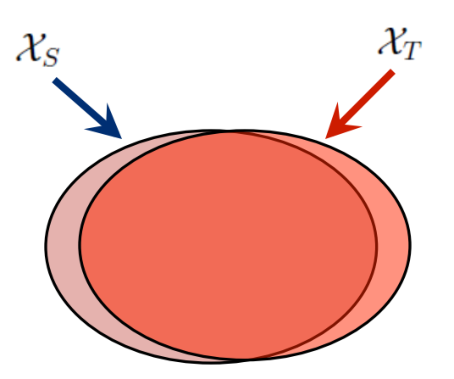
\includegraphics[scale=0.5]{./figures/fig-feature.pdf}
	\caption{特征选择法示意图}
	\label{fig-feature}
\end{figure}

\subsection{核心方法}

这这个领域比较经典的一个方法是发表在2006年的ECML-PKDD会议上,作者提出了一个叫做SCL的方法(Structural Correspondence Learning)~\cite{blitzer2006domain}。这个方法的目标就是我们说的,找到两个领域公共的那些特征。作者将这些公共的特征叫做Pivot feature。找出来这些Pivot feature,就完成了迁移学习的任务。

\begin{figure}[htbp]
	\centering
	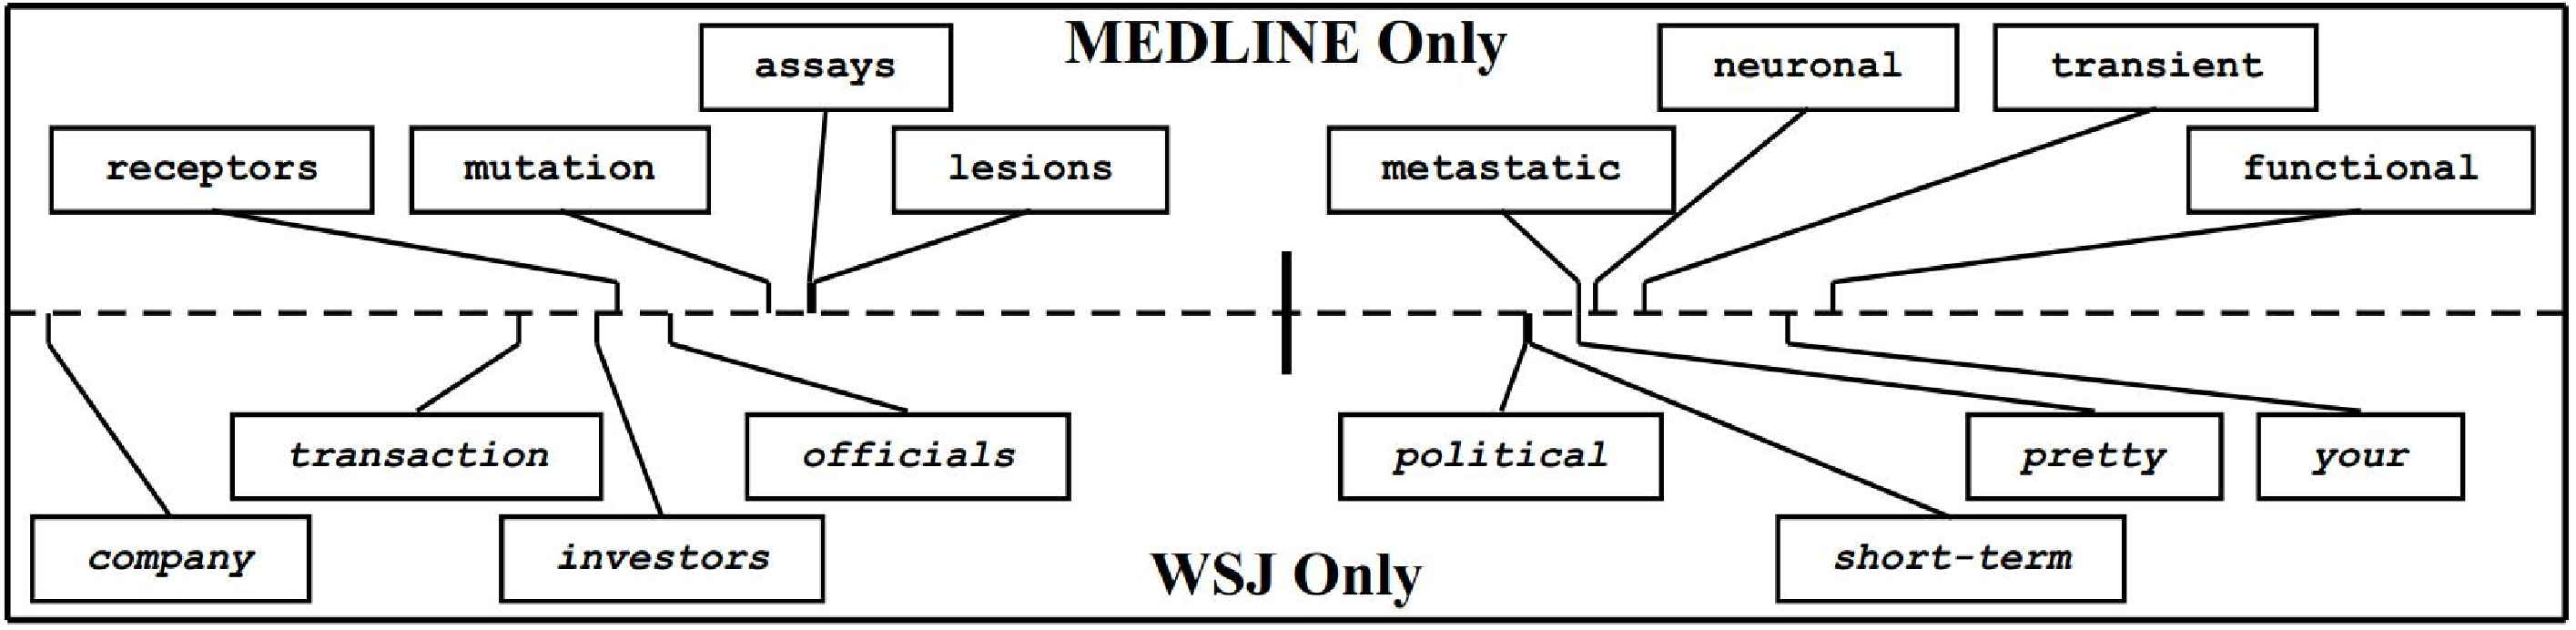
\includegraphics[scale=0.3]{./figures/fig-feature-pivot.pdf}
	\caption{特征选择法中的Pivot feature示意图}
	\label{fig-feature-pivot}
\end{figure}

图~\ref{fig-feature-pivot}形象地展示了Pivot feature的含义。Pivot feature指的是在文本分类中,在不同领域中出现频次较高的那些词。


\subsection{扩展}

SCL方法是特征选择方面的经典研究工作。基于SCL,也出现了一些扩展工作。

\begin{itemize}
	\item Joint feature selection and subspace learning~\cite{gu2011joint}:特征选择+子空间学习
	\item TJM (Transfer Joint Matching)~\cite{long2014transfer}: 在优化目标中同时进行边缘分布自适应和源域样本选择
	\item FSSL (Feature Selection and Structure Preservation)~\cite{li2016joint}: 特征选择+信息不变性
\end{itemize}

\subsection{小结}

\begin{itemize}
	\item 特征选择法从源域和目标域中选择提取共享的特征,建立统一模型
	\item 通常与分布自适应方法进行结合
	\item 通常采用稀疏表示$||\mathbf{A}||_{2,1}$实现特征选择
\end{itemize}
